\usepackage[utf8]{inputenc}
\usepackage{array}
\documentclass[12pt]{report}
% Bar chart drawing library 
\usepackage{pgfplots} 
% Curve
\usepackage{graphicx}
\graphicspath{ {./images/} }
\usepackage{mathtools}
\usepackage{amsmath}
\usepackage[a4paper, total={7in, 10in}]{geometry}


\usepackage{pgfplots}
\pgfplotsset{width=10cm,compat=1.9}

% We will externalize the figures
\usepgfplotslibrary{external}
\tikzexternalize




\title{A Comprehensive Guide to the History and Solutions to the Brachistochrone Problem}
\author{Zayaan Mulla}
\date{December 2021}

\begin{document}

\maketitle

\tableofcontents

\chapter{Foreword}
Whilst attempting to find a topic of a mathematical nature to base my EPQ upon, I discovered that most of the interesting mathematics conducted and published through various journals relied on the assumption that the reader would have been exposed to similar research before, and that the reader may also have been involved in higher level mathematics themselves, at university or beyond. This made the papers mostly inaccessible to someone without an understanding of university level mathematics. In the case of the Brachistochrone Problem, I found that most of the mathematics published on the topic could be explained carefully such that a high school student may understand it, but it needed to be presented in such a way that it explained each concept from first principles, which was not evident throughout any of the papers I read on the topic.
\\\\
The purpose of this project is to present the mathematics of the Brachistochrone Problem, including the solutions, as well as any mathematics related to deriving the solutions themselves, in a more accessible form such that the guide may be comprehended by an advanced high school students, who has been exposed to calculus. Upon providing some historical and mathematical context to the problem, the guide will go through a few of the approaches taken to solve the problem, including the Calculus of Variations. The aim is to ensure that each step taken to solve the problem is explained carefully and that the motivations behind each proof are deliberated over. We will begin from first principles and derive each result from scratch so that the pre-requisite knowledge required by the reader is minimal (basic calculus and trigonometry, partial differentiation and multivariate chain rule).
\\\\
I hope you enjoy!

\chapter{Introduction to the Brachistochrone Problem}
\section{Chapter Overview}
The focus of this chapter is to provide the reader with some historical context with regards to the origins of the Brachistochrone problem, as well as to provide them with an introduction to some of the methods used to solve the problem.
\\\\
We will first go over the actual definition of the problem statement itself, and then go onto providing a brief history of the problem, detailing the involvement of some of the most influential Mathematicians in history, and their roles in solving this problem.
\section{What is the Brachistochrone Problem?}
The problem states the following:
\\
\\
"Given 2 points, A and B, in an \(x-y\) plane, what is the curve traced out by a point acted on only by gravity, which starts at A and reaches B in the shortest time?" [1]
\\
\\
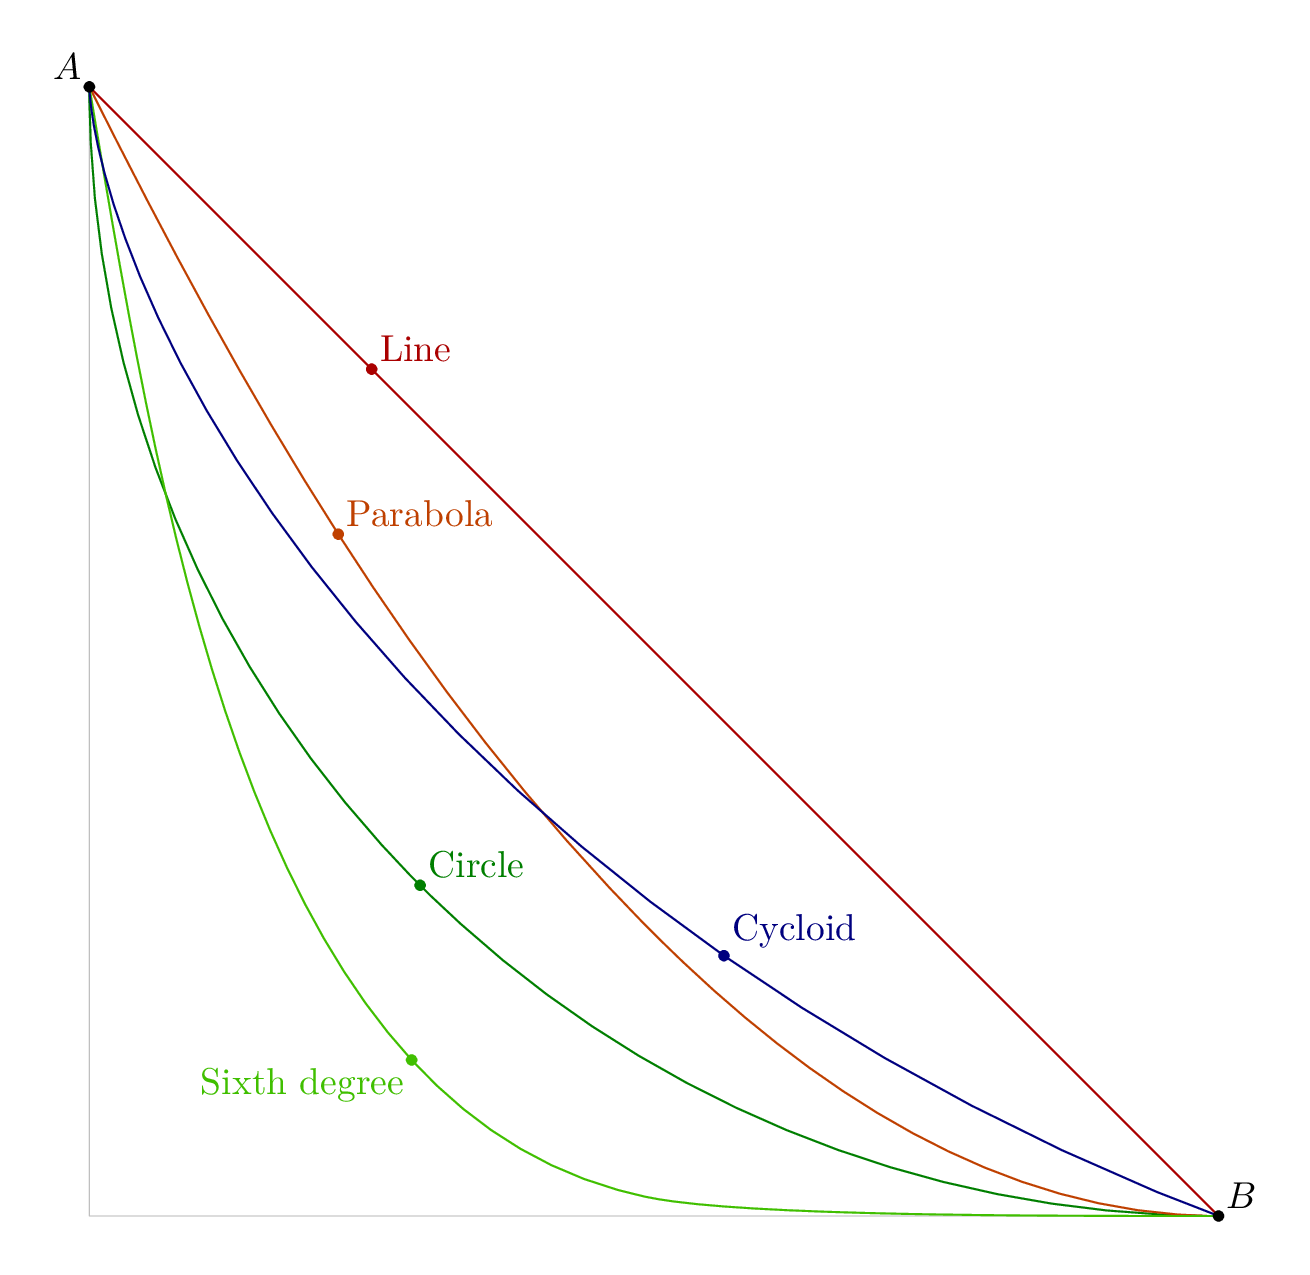
\includegraphics[width=9cm, height=7cm]{EPQ - VC/tPtMm.png} [2]
\\
Figure 1
\\
\\
The problem is a different sort of optimization problem as instead of asking for a point on a curve that minimizes the function, it is asking for a curve that minimizes the function. This is where the Calculus of Variations is important, as it is the method used to solve optimization problems of this nature. Before we get into that however, we will first explore some of the history behind the problem as well as Galileo Galilei's attempt at solving it before the problem was even posed by Johann Bernoulli. [3]

\section{A Brief History}
Before the Brachistochrone problem was posed by Johann Bernoulli in 1696, Galileo had worked on the problem in his 'Discourse on Two New Sciences', his famous last book in which he covers much of his work in Physics over the preceding 30 years. His original problem was to find the shape of the curve from point A to a point B on the \(x-y\) plane such that the distance from A to B is minimised. He arrived at the correct conclusion in that the shape taken by this curve would be a straight line. Interested in solving similar path optimization problems, he then attempted to find the shortest path between the two points, such that if a ball (modelled as a particle) was dropped at A, it would reach B in the fastest time. This was of course the Brachistochrone Problem, only he didn't know it yet. He discovered that it would reach B more quickly if it were to travel along 2 straight line segments, suppose AC and CB, where C is a point on a circle. Although this was correct, his error lied in his deduction from this that the path of fastest descent from A to B then would be an arc of a circle, which happened to be incorrect. [1]
\\
\\
Lets fast forward to 1696, and Johann Bernoulli has published the Brachistochrone Problem as a challenge in 'Acta Eruditorum', A Mathematical Journal coincidentally edited by Leibniz. The thing is, Johann Bernoulli had already solved the problem, taking him 2 weeks, through what he thought was an exceptionally elegant method. All he really wanted to show the world that he was the best Mathematician of his generation. Another intention of his was to lure Isaac Newton into solving the problem. Newton at the time was retired from Mathematics and was employed as Warden of the Royal Mint. Upon hearing of the problem, it is said that Newton came home one day at 4 in the afternoon, tired after returning from the Royal Mint, and proceeded to stay up till 4 in the morning until he solved it. Newton sent his solution to his friend, Charles Montague, President of the Royal Society at the time. Montague later revealed that the challenge did not please Newton and that he stated "I do not love to be dunned (pestered) and teased by foreigners about mathematical things". Newton's solutions was published anonymously through the Royal Society in the 'Philosophical Transactions of the Royal Society' in January of 1697. After examining the solution, Johann Bernoulli is said to have exclaimed "I recognise the lion by its claw", in reference to recognizing the work as Newton's. In the end, the problem was solved by Johann, and his brother Jacob Bernoulli, as well as famous mathematicians L'hopital, Leibniz and of course, Newton.

\chapter{Johann Bernoulli's Proof}
\section{Chapter Overview}
We're going to slightly divert our attention from the Brachistochrone problem for the next couple of sections in order to explain some key concepts to fully understand Johann Bernoulli's proof of the Brachistochrone problem. We will first begin with Fermat's Principle of Least Time and how it is used in deriving Snell's Law, which is a key part of Bernoulli's solution. We will then go onto deriving the parametric equations of a cycloid, which will be of use to us when it comes to interpreting the solution when we get there. We will then show how Snell's Law is related to the parametric equations of a cycloid and finally tie this all together through Johann Bernoulli's proof of the Brachistochrone problem.
\section{Deriving Snell's Law}
Fermat's Principle states:
\\
\\
"light rays follow paths of least time" [5]
\\
\\
This can be used to derive the Law of Refraction, also known as Snell's Law, which will aid us in communicating Johann Bernoulli's proof.
\\
\\
For those of you that don't know, Snell's Law is, of course:
\\
\\
\(n_{1} \sin{\theta_{1}} = n_{2} \sin{\theta_{2}}\),
\\
\\
where \(n\) is the incident or refractive index respectively and \(\theta\) is the angle of incidence or refraction, respectively.
\\
\\
We can begin proving this by considering the following diagram:
\\
\\
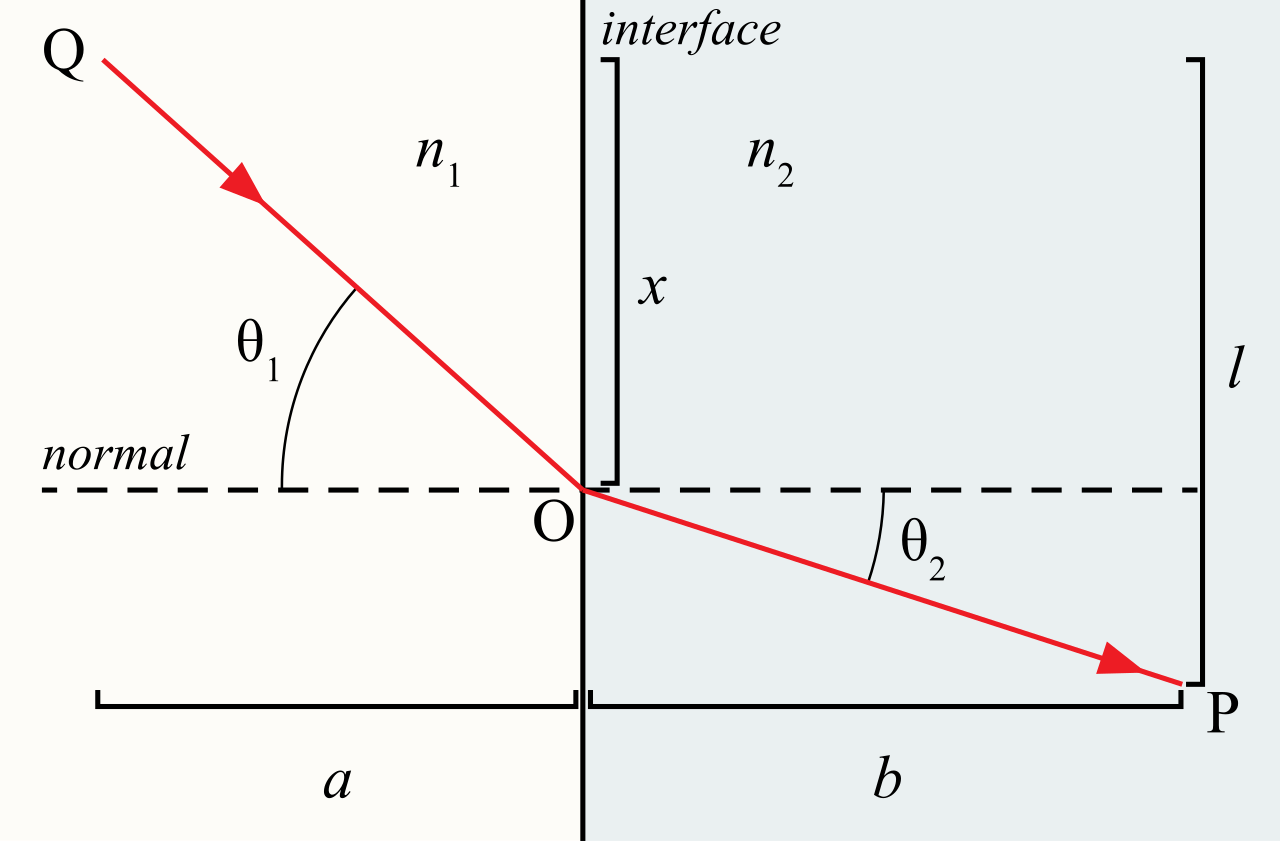
\includegraphics[width=9cm, height=7cm]{EPQ - VC/Snell'sL.png}
\\
\\
By Pythagoras' Theorem, we can let \(|QO|= \sqrt{x^2 + a^2}\) and \(|OP| = \sqrt{(l-x)^2+b^2}\)
\\
\\
Now by letting the speed in the medium above the normal be \(v_{1}\) and the speed in the medium below the normal be \(v_{2}\), and given \(time=\frac{distance}{speed}\), we can write the time taken to get from Q to O, and O to P, as \(\frac{\sqrt{x^2 + a^2}}{v_{1}}\) and \(\frac{\sqrt{(l-x)^2+b^2}}{v_{2}}\) respectively.
\\
\\
Therefore we can let the total time taken to get from Q to P be \(T\), where \(T=\frac{\sqrt{x^2 + a^2}}{v_{1}}+\frac{\sqrt{(l-x)^2+b^2}}{v_{2}}\)
\\
\\
By Fermat's Principle, we are dictated to minimise the time taken to get from Q to P. Given that a straight line is trivially the shortest path between both points, we can consider the possibility of the light ray travelling normal to the surface, which would mean that it would follow the path of a straight line without experiencing any refraction at all. Therefore, if we minimise x, we are minimising the path length, and hence the time taken to get from Q to P.
\\
\\
Assuming this logic, we can take \(\frac{dt}{dx}\) and set it \(=0\)
\\
\\
\implies \(\frac{d}{dx}(\frac{\sqrt{x^2 + a^2}}{v_{1}}+\frac{\sqrt{(l-x)^2+b^2}}{v_{2}}) = 0\)
\\
\\
\implies \(\frac{x}{v_{1}\sqrt{x^2 + a^2}}-\frac{(l-x)}{v_{2}\sqrt{(l-x)^2+b^2}} = 0\)
\\
\\
Now by inspecting the 2 triangles produced by the diagram, we see that \(\sin{\theta_{1}} = \frac{x}{|QO|}\)
\\
\\
\implies \(\sin{\theta_{1}} = \frac{x}{\sqrt{x^2 + a^2}}\)
\\
\\
Similarly, we can see that \(\sin{\theta_{2}} = \frac{l-x}{|OP|}\)
\\
\\
\implies \(\sin{\theta_{2}} = \frac{l-x}{\sqrt{(l-x)^2+b^2}}\)
\\
\\
Therefore, by substituting for \(\sin{\theta_{1}}\) and \(\sin{\theta_{2}}\) in \(\frac{dt}{dx} = 0\),
\\
\\
We end up with \(\frac{\sin{\theta_{1}}}{v_{1}} - \frac{\sin{\theta_{2}}}{v_{2}}=0\)
\implies \(\frac{\sin{\theta_{1}}}{v_{1}} = \frac{\sin{\theta_{2}}}{v_{2}}\)
\\
\\
We can now consider the fact that the speed of a particle in a medium, \(v\), is given by \(v = \frac{c}{n}\), where n, the refractive index of the medium, describes how fast light travels through the material, and c is the speed of light = \(3 \times 10^8 ms^{-1}\).
\\
\\
Using this, we can rewrite \(v_{1}\) and \(v_{2}\) in terms of \(c\), and \(n_{1}\) and \(n_{2}\), respectively, as follows:
\\
\\
\(v_{1} = \frac{c}{n_{1}}\), \(v_{2} = \frac{c}{n_{2}}\)
\\
\\
Substituting this back into \(\frac{\sin{\theta_{1}}}{v_{1}} = \frac{\sin{\theta_{2}}}{v_{2}}\), we end up with:
\\
\\
\(\frac{\sin{\theta_{1}}}{\frac{c}{n_{1}}} = \frac{\sin{\theta_{2}}}{\frac{c}{n_{2}}}\)
\\
\\
\implies \(n_{1}\sin{\theta_{1}} = n_{2}\sin{\theta_{2}}\),
\\
\\
which is of course, Snell's Law. [6]

\section{Parametric Equations of a Cycloid}
Given that the solution of the Brachistochrone happens to be the curve created by a Cycloid, it would only make sense for us to derive the parametric equations of a Cycloid before we proceed to presenting any proofs, in order for us to recognise the solution once we get there.
\\
\\
We can note that a Cycloid is the curve generated by a point on the circumference of a circle that rolls along a straight line.
\\
\\
They end up being:
\\
\\
\(x = a(\theta-\sin{\theta})\) and \(y = a(1-\cos{\theta})\)
\\
\\
To show this we can consider the following diagram [15]:
\\
\\

\begin{center}
  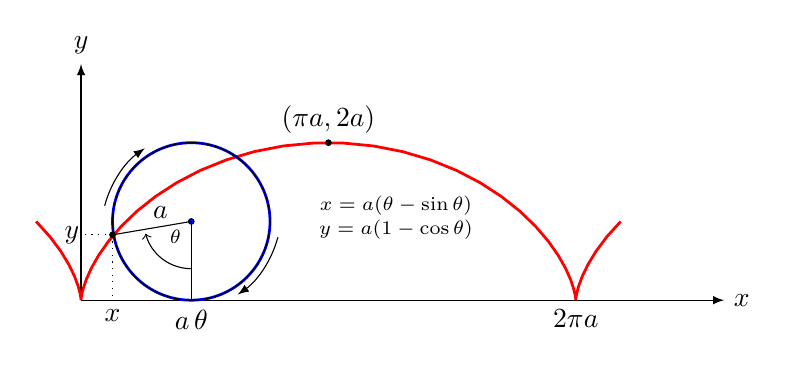
\begin{tikzpicture}
  \coordinate (O) at (0,0);
  \coordinate (A) at (0,3);
  \def\r{1} % radius
  \def\c{1.4} % center
  \coordinate (C) at (\c, \r);


  \draw[-latex] (O) -- (A) node[anchor=south] {$y$};
  \draw[-latex] (O) -- (2.6*pi,0) node[anchor=west] {$x$};
  \draw[red,domain=-0.5*pi:2.5*pi,samples=50, line width=1] 
       plot ({\x - sin(\x r)},{1 - cos(\x r)});
  \draw[blue, line width=1] (C) circle (\r);
  \draw[] (C) circle (\r);

  % coordinate x 
  \def\x{0.4} % coordinate x
  \def\y{0.83} % coordinate y
  \def\xa{0.3} % coordinate x for arc left
  \def\ya{1.2} % coordinate y for arc left
  \coordinate (X) at (\x, 0 );
  \coordinate (Y) at (0, \y );
  \coordinate (XY) at (\x, \y );

  \node[anchor=north] at (X) {$x$} ;

  % draw center of circle
  \draw[fill=blue] (C) circle (1pt);

  % draw radius of the circle
  \draw[] (C) -- node[anchor=south] {\; $a$} (XY);

  % bottom of circle, radius to the bottom
  \coordinate (B) at (\c, 0);
  \draw[] (C) -- (B) node[anchor=north] {$a \, \theta$};

  % projections of point XY
  \draw[dotted] (XY) -- (X);
  \draw[dotted] (XY) -- (Y) node[anchor=east, xshift=1mm] {$\quad y$};

  % arc theta
  % start arc
  \coordinate (S) at (\c, 0.4);
  \draw[->] (S) arc (-90:-165:0.6);
  \node[xshift=-2mm, yshift=-2mm] at (C) {\scriptsize $\theta$};

  % arc above
  \coordinate (AA) at (\xa, \ya);
  \draw[-latex, rotate=25] (AA) arc (-220:-260:1.3);

  % arc below
  \def\xb{2.5} % coordinate x for arc bottom
  \def\yb{0.8} % coordinate y for arc bottom
  \coordinate (AB) at (\xb, \yb);
  \draw[-latex, rotate=-10] (AB) arc (-5:-45:1.3);



  % XY dot
  \draw[fill=black] (XY) circle (1pt);


  % top label
  \coordinate (T) at (pi, 2);
  \node[anchor=south] at (T)  {$(\pi a, 2 a )$} ;
  \draw[fill=black] (T) circle (1pt);

  % equations
  \coordinate (E) at ( 4,1.2);
  \coordinate (F) at ( 4,0.9);
  \node[] at (E) {\scriptsize $x=a(\theta - \sin \theta)$};
  \node[] at (F) {\scriptsize $y=a(1 - \cos \theta)$};

  % label 2pi a
  \coordinate (TPA) at (2*pi, 0);
  \node[anchor=north] at (TPA) {$2 \pi a$};


  \end{tikzpicture}
\end{center}
\\
\\
For completeness sake's, I will explain the trigonometry conducted through the diagram, leading to the equations of a Cycloid.
\\
\\
We can begin by labelling an arbitrary point on the Cycloid, \((x, y)\), and the radius of the circle, \(a\). We can then let the angle of the sector between the point \((x, y)\), and the point \(x = a\theta\), be \(\theta\), where  \(a\theta\) is both the length of the sector, and a point on the circle that lies on the \(x\) axis.
\\
\\
We can then consider the distance between \(x, a\theta\) to be = \(a\sin{\theta}\), due to the right angled triangle formed by drawing a perpendicular bisector from \((x, y)\) to the line \(x = a\theta\). This is due to letting the radius of the circle, \(a\) = the hypotenuse of the triangle formed, and then conducting simple trigonometry to find the length of the opposite (to the angle \(\theta\) which is indicated) side of the triangle to be \(a\sin{\theta}\).
\\
\\
We can write this as \(a\theta - x = a\sin{\theta}\), which rearranges to give
\\
\\
\(x = a\theta - a\sin{\theta}\)
\\
\implies \(x = a(\theta -\sin{\theta})\), which is our desired equation for \(x\).
\\
\\
Similarly for y, we can consider the same right angled triangle formed by drawing a perpendicular bisector from \((x, y)\) to the line \(x = a\theta\). From this we can see that \(\cos{\theta} = \frac{a-y}{a}\), as \(a\) is the radius of the circle, so \(y\) must be subtracted from it to give the length of the adjacent side (to the angle \(\theta\) which is indicated) of the triangle. Also given that \(a\) is the radius of our circle, it can form the hypotenuse of the triangle we are inspecting, which leads us to our value of \(\cos{\theta}\).
\\
\\
Therefore, by rearranging \(\cos{\theta} = \frac{a-y}{a}\), 
\\
\\
\(y = a-a\cos{\theta}\)
\\
\implies \(y = a(1-\cos{\theta})\), which is our desired equation for \(y\).
[7] 

\section{Bernoulli's Proof}
Johann Bernoulli's proof was the product of an ingenious thought experiment involving a non uniform optical medium, which decreases in refractive index, and hence optical density, as you go down the medium. Considering this medium as infinite, he made use of the principle of conservation of energy, and Fermat's principle of least time, and hence Snell's Law, to reason about the problem. Using some geometrical insights and the idea that the speed of light would increase as it goes from a medium with a higher to lower optical density, Bernoulli was able to derive a differential equation of the form:
\\
\\
\(\frac{dy}{dx} = \sqrt{\frac{C-y}{y}}\)
\\
\\
Instead of solving the differential equation via conventional means, he immediately identified it to be the differential equation of a Cycloid, and went on to publish the solution in Acta Eruditorum in May of 1697. For the sake of completeness however, we will derive the parametric equations representing our solution by employing a clever trigonometric substitution to solve the differential equation ourselves.
\\
\\
We can begin the proof by considering the following diagram:
\\
\\
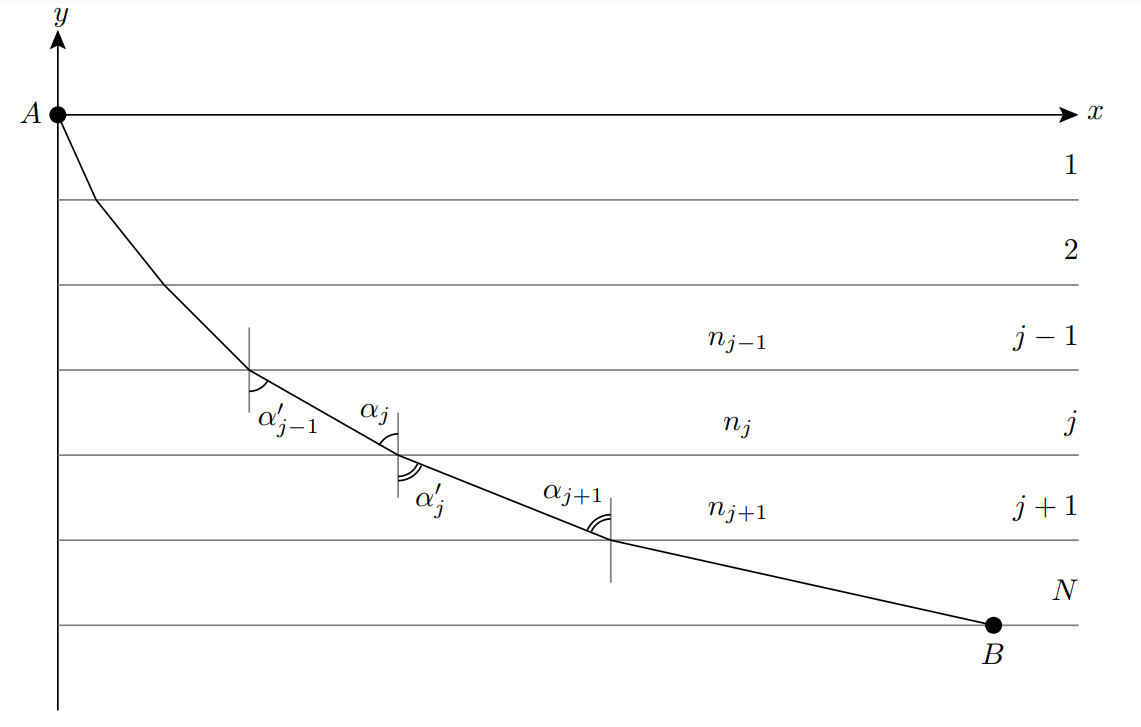
\includegraphics[width=11cm, height=9cm]{EPQ - VC/SLGradientt.png} [6]
\\
\\
The diagram here illustrates a path followed by a particle from A to B, which follows Fermat's principle of least time, and hence is the shortest possible path from A to B. The diagram is divided into layers, each of a different refractive index. This means that the particle makes an angle to the normal.
\\
\\
Through this we note that by Snell's Law,
\\
\\
\(n_{j-1}\sin{\alpha_{j-1}} = n_{j}\sin{\alpha_{j}} = n_{j+1}\sin{\alpha_{j+1}} = ...\)
\\
\\
\implies \(n\sin{\alpha} = C\), where \(C\) is some arbitrary constant, \(n\) is the refractive index of that medium, and \(c\) is the speed of light.
\\
\\
Given \(n=\frac{c}{v}\)
\\
\\
\implies \(\frac{c}{v}\sin{\alpha} = C\)
\\
\\
\implies \(\frac{\sin{\alpha}}{v} = C\), as \(c\) is a constant and when divided through on both sides, results on another constant on the RHS.
\\
\\
Therefore, by now using the principle of conservation of energy, such that
\\
\\
\(\frac{1}{2}mv^2 = mg\Delta h\), where \(\Delta h\) = the height the particle falls in that medium.
\\
\\
\implies \(v = \sqrt{2g\Delta h}\)
\\
\\
We can rewrite \(\frac{\sin{\alpha}}{v} = C\) as \(\frac{\sin{\alpha}}{\sqrt{2g\Delta h}} = C\)
\\
\\
\implies \(\frac{\sin{\alpha}}{\sqrt{\Delta h}} = C\), as \(\sqrt{2g}\) is a constant, and when multiplied through on both sides, results in a constant value on the RHS.
\\
\\
As \(\Delta h\) = the height the particle falls in that medium = \(y\),
\\
\implies \(\frac{\sin{\alpha}}{\sqrt{y}} = C\)
\\
\\
We can now consider the right angled triangle formed as the particle enters another medium, as illustrated by the diagram:
\\
\\
\usetikzlibrary{decorations.pathreplacing}

      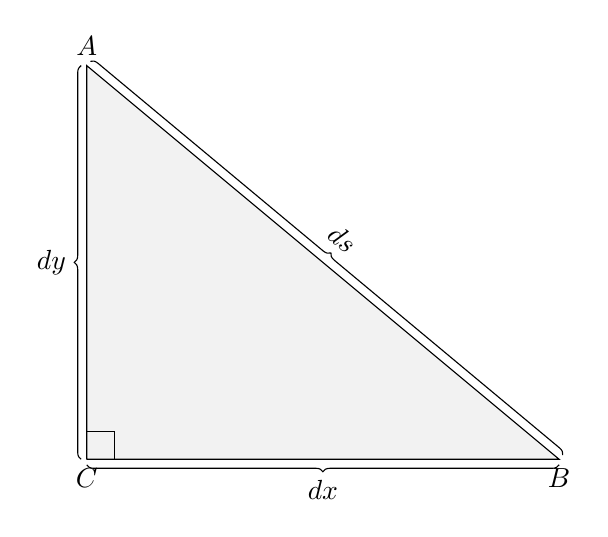
\begin{tikzpicture}
% Draw the triangle
        \draw[fill=gray!10]  (0, 0) coordinate (C) 
        -- (0,5) coordinate (A) 
        -- (6,0) coordinate (B) 
        -- (0, 0);
       \draw[decoration={brace,mirror,raise=2pt},decorate] 
         (C) -- node[below=4pt] {$dx$} (B); 
       \draw[decoration={brace,mirror,raise=2pt},decorate] 
         (B) -- node[above=4pt,sloped] {$ds$} (A); 
       \draw[decoration={brace,mirror,raise=2pt},decorate] 
         (A) -- node[left=4pt] {$dy$} (C); 

       \draw (0,10pt) -- ++(10pt,0) -- ++(0,-10pt);
% Draw nodes
        \node at (A)[anchor=south] {$A$};
        \node at (B)[anchor=north] {$B$};
        \node at (C)[anchor=north] {$C$};
        
        
      \end{tikzpicture}
\\
\\
We can let the vertical distance travelled by the particle in the medium be \(dy\), and the horizontal distance \(dx\). This will let us find the total distance travelled by the particle in a medium, \(ds\) by Pythagoras' theorem.
\\
\\
\(ds = \sqrt{dx^2+dy^2}\)
\\
\\
\(ds = \sqrt{dx^2}\sqrt{1+(\frac{dy}{dx})^2}\)
\\
\\
\(ds = \sqrt{1+y'^2}dx\)
\\
\\
We can assume \(\alpha\) to be the angle at A, and hence as \(\sin{\theta} = \frac{opposite}{hypotenuse}\), \(\sin{\alpha} = \frac{dx}{ds} = \frac{dx}{\sqrt{1+y'^2}dx}\)
\\
\\
\implies \(\sin{\alpha} = \frac{1}{\sqrt{1+y'^2}}\)
\\
\\
We can now rewrite \(\frac{\sin{\alpha}}{\sqrt{y}} = C\) in terms of only \(y\) and \(y'\) as follows:
\\
\\
\(\frac{\frac{1}{\sqrt{1+y'^2}}}{\sqrt{y}} = C\)
\\
\\
\implies \(\frac{1}{\sqrt{y(1+y'^2)}} = C\) \implies \(\sqrt{y(1+y'^2)} = \frac{1}{C}\)
\\
\\
As \(C\) is an arbitrary constant, we can let \(\frac{1}{C} = C_{1}\), and also \(C^2 = C_{1}\)
\\
\\
Therefore, \(y(1+y'^2) = C_{1}\)
\\
\\
We can rearrange terms to make \(y'\) the subject as follows:
\\
\\
\(1+y'^2 = \frac{C_{1}}{y}\)
\\
\implies \(y'^2 = \frac{C_{1}}{y}-1 = \frac{C_{1}-y}{y}\)
\\
\implies \(y' = \sqrt{\frac{C_{1}-y}{y}}\)
\\
\\
And hence, \(\frac{dy}{dx} = \sqrt{\frac{C_{1}-y}{y}}\)
\\
\\
We can then form a differential equation by separating the variables as follows:
\\
\\
\({dx} = \sqrt{\frac{y}{C_{1}-y}}{dy}\)
\\
\\
Then by integrating both sides, we get
\\
\\
\(x + C_{2} = \int (\sqrt{\frac{y}{C_{1}-y}})dy\)
\\
\\
We can now consider using the substitution \(y = C_{1}\sin^2{\theta}\), 
\\
where \(\frac{dy}{d\theta} = 2 \cdot C_{1}\sin{\theta}\cos{\theta}\)
\\
\\
\implies\(dy = 2 \cdot C_{1}\sin{\theta}\cos{\theta} d\theta\)
\\
\\
Then by using this substitution in the RHS, we can form an integral such that
\\
\\
\(\int (\sqrt{\frac{y}{C_{1}-y}})dy = \int(\sqrt{\frac{C_{1}\cdot \sin^2{\theta}}{C_{1}-C_{1}\cdot \sin^2{\theta}}} \cdot 2 \cdot C_{1}\sin{\theta}\cos{\theta}) d\theta\)
\\
\\
By cancelling out \(C_{1}\) inside of the square root from the numerator and denominator, as well as making use of the fact that \(1-\sin^2{\theta} = \cos^2{\theta}\), the RHS simplifies to:
\\
\\
\(\int(\sqrt{\frac{\sin^2{\theta}}{\cos^2{\theta}}} \cdot 2 \cdot C_{1}\sin{\theta}\cos{\theta}) d\theta\)
\\
\\
\implies \(\int(\frac{\sin{\theta}}{\cos{\theta}} \cdot 2 \cdot C_{1}\sin{\theta}\cos{\theta}) d\theta\)
\\
\\
Then by cancelling out \(\cos{\theta}\) from the numerator and denominator, the integral simplifies to:
\\
\\
\(\int(\sin{\theta} \cdot 2 \cdot C_{1}\sin{\theta}) d\theta\)
\\
\\
By taking out constant factors, we can rewrite this as:
\\
\\
\(2C_{1}\int (\sin^2{\theta}) d\theta\)
\\
\\
Given \(\sin^2{\theta} = \frac{1}{2}\cdot (1-\cos{2\theta})\), from the double angle formulae,
\\
\\
\implies \(2C_{1}\int (\frac{1}{2}\cdot (1-\cos{2\theta})) d\theta\)
\\
\\
\implies \(C_{1}\int (1-\cos{2\theta}) d\theta\)
\\
\\
We can now integrate this to give us \(C_{1} (\theta-\frac{1}{2}\sin{2\theta})\)
\\
\\
By recalling the original equation before the substitution, \(x + C_{2} = \int (\sqrt{\frac{y}{C_{1}-y}})dy\), we can now rewrite this as follows:
\\
\\
\(x + C_{2} = C_{1} (\theta-\frac{1}{2}\sin{2\theta})\)
\\
\\
\implies \(x = C_{1} (\theta-\frac{1}{2}\sin{2\theta}) - C_{2}\)
\\
\\
From the substitution used to solve the integral, we can also recall \(y\) to be equal to \(C_{1}\sin^2{\theta}\)
\\
\\
\implies \(y =\frac{C_{1}}{2} \cdot (1-\cos{2\theta}) \), from the double angle formulae.
\\
\\
Therefore we can define the parametric equations of the curve traced out by the particle on its path such that the time taken from a to b is minimised, to be as follows:
\\
\\
\(x = C_{1} (\theta-\frac{1}{2}\sin{2\theta}) - C_{2}\)
\\
\\
\(y =\frac{C_{1}}{2} \cdot (1-\cos{2\theta}) \)
\\
\\
Where \(C_{1}\) and \(C_{2}\) are of course arbitrary constants which can be determined by the boundary conditions.
\\
\\
These set of parametric equations, as shown in the previous subchapter, are known to resemble those of the Cycloid. Hence we can conclude that the final shape of the path taken by the particle, subject to the constraints outlined earlier is the shaped traced out by a point on a Cycloid moving moving between the 2 points.
\\
\\
We can further consult the diagram below for a more geometrical perspective of the solution:
\\
\\
\begin{tikzpicture}
\draw[->] (0,0) -- (0,3);
\draw[->] (0,0) -- (2.6*pi,0);
\draw[red,domain=-0.5*pi:2.5*pi,samples=50] plot ({\x - sin(\x r)},{1 - cos(\x r)});
\end{tikzpicture} [4]
\\
\\
[8], [14]
\chapter{The Calculus of Variations}
\section{Chapter Overview}
Throughout this chapter we will aim to introduce the Calculus of Variations, as a method of solving the Brachistochrone Problem. The first section will begin with the motivations behind the Calculus of Variations, including a brief history and a generalization of the foundational principle of the Calculus of Variations itself. We will then go onto deriving the Euler-Largange equation, the fundamental equation of the Calculus of variations. The Euler-Lagrange equation is a system of second order ordinary differential equations, whose solutions unveil the stationary functions of any given functional. That may not make much sense right now but it will when we get to it. It is essentially an equation that used to derive solutions to various path minimization problems, including but not limited to the Brachistochrone Problem. Upon deriving the Euler-Lagrange equation, we will present an application of it on a problem we already know the answer to, the path of shortest distance. This will help in understanding how to apply the the Euler-Largange equation, via a simpler problem. In the penultimate section of the chapter we will derive something known as the Beltrami Identity; a reduced form of the Euler-Largange equation which will simplify our solution to the Brachistochrone Problem, which we will present in full, tying all the ideas presented in the previous sections, in the final section.
\section{Motivations}
In 1755, A man named Lagrange was working, age 19, on a problem known as the Tautochrone Problem. This was a variation of the Brachistochrone Problem which consisted of finding the curve for which the time it takes for a mass to slide frictionlessly down along to its lowest point on the curve is independent of where the mass started to slide along the curve. [9] The solution to this problem also happens to be a Cycloid, but we wont get into the details as it's outside the scope of this guide. Coming back to Lagrange, he goes onto publish a paper on a method of analysing problem such as this from an analytic standpoint, contrasting with Euler's geometric approach. Euler had worked on the Brachistochrone Problem at around 1733, and was so impressed with Lagrange's method that he abandoned his own to use Lagrange's. He even waited for Lagrange to catch up before finally publishing a paper on the Calculus of Variations in 1756. The paper provided a framework for Fermat's principle, the Tautochrone and the Brachistochrone problem, and many other path minimisation problems. [4]
\\
\\
Now, what does the Calculus of Variations actually do? Let's look back to differential calculus, where the purpose is to find a point on a curve that minimises that function. In the Calculus of Variations, it's all about finding a function that minimises a functional, where a functional is the whole family of possible curves subject to constraints. Think about the Brachistochrone Problem for a second. What the problem is really asking us is what is the function, out of all possible functions, that minimises the time taken to travel between the 2 points, A and B.
\\
\\
Writing this out Mathematically:
\\
\\
since \(time=\frac{distance}{speed}\), \(dt=\frac{ds}{v(x,y)}\), where:
\\
\\
\(dt\) = the time taken to get from A to B,
\\
\\
\(ds\) = the distance from A to B = \(\sqrt{dx^2 + dy^2}\),
\\
\\
and \(v(x,y)\) = the velocity at coordinates \((x,y)\)
\\
\\
Therefore if we're looking to minimise \(dt\), we must form an integral \(T\), for which:
\\
\\
Given \(ds\) = \(\sqrt{dx^2 + dy^2}\) = \(\sqrt{1 + \frac{dy^2}{dx^2}} dx\),
\\
\\
\(T=\int\limits_a^b\frac{\sqrt{1 + \frac{dy^2}{dx^2}}dx}{v(x,y)}\)
\\
\\
Where the limits, a and b, represent the x coordinates of their respective points, a and b.
\\
\\
The problem of minimising T is of course, the Brachistochrone Problem, and will require the use of techniques presented in the Calculus of Variations to compute.
\\
\\
By inspecting the example, in general, what the Calculus of Variations seeks to find is \(f(x)\), such that
\\
\\
\(I[f] = \int\limits_a^b\ F(x, y, \frac{dy}{dx})dx\) is stationary
\\
\\
This is also known as the foundational principle of the Calculus of Variations.
\section{Derivation of the Euler-Lagrange Equation}
The Euler-Lagrange equation is a differential equation which allows us to find the stationary functions of a functional (functions of a function), or in other words, helps us to solve problems in the Calculus of Variations of the form
\\
\\
\(I[f] = \int\limits_a^b\ F(x, y, \frac{dy}{dx})dx\), 
\\
\\
which is exactly what we introduced at the end of the last subchapter.
\\
\\
It was described by Hamilton as a scientific poem.
\\
\\
We will be deriving the Euler-Lagrange equation using some calculus (including the chain rule for several variables and some integration by parts) and will demonstrate an application of it on a simple shortest path problem in the next subchapter before continuing on to solving the Brachistochrone Problem through the Calculus of Variations.
\\
\\
We can begin the derivation by considering \(y(x)\). We'll let this be the shortest path from \((x_{1}, y_{1})\) to \((x_{2}, y_{2})\), where they are the start and endpoints of the graph respectively.
\\
\\
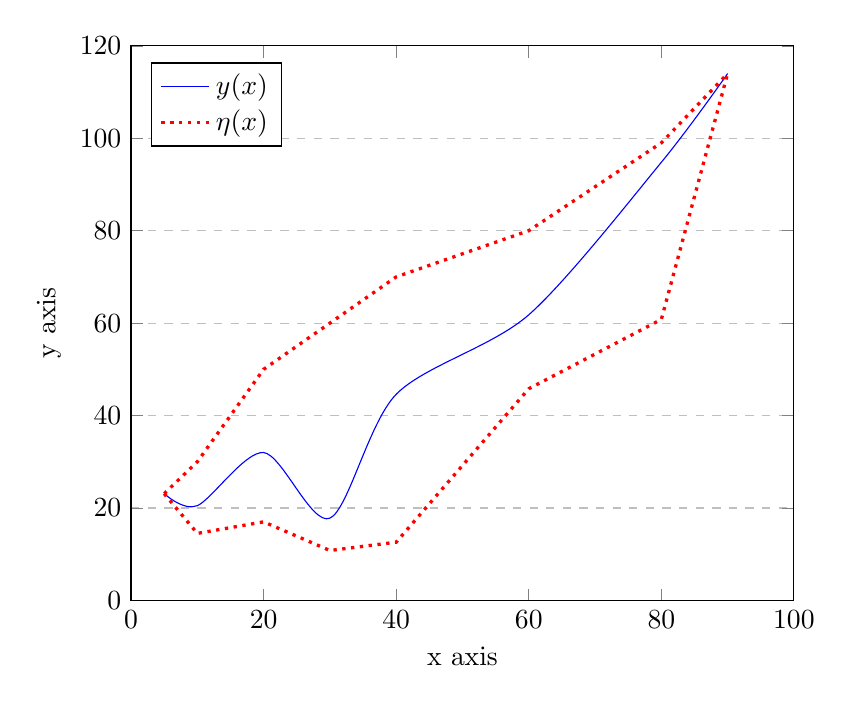
\begin{tikzpicture}
\begin{axis}[
    xlabel={x axis},
    ylabel={y axis},
    xmin=0, xmax=100,
    ymin=0, ymax=120,
    xtick={0,20,40,60,80,100},
    ytick={0,20,40,60,80,100,120},
    legend pos=north west,
    ymajorgrids=true,
    grid style=dashed,
]

\addplot[smooth]
    [color = blue]
    coordinates {
    (5,23.1)(10,20.5)(20,32)(30,17.8)(40,44.6)(60,61.8)(80,94.8)(90,114)
    };
    
\addplot[very thick, dotted][color = red]
    coordinates {
    (5,23.1)(10,30)(20,50)(30,60)(40,70)(60,80)(80,99)(90,114)
    };
    \legend{\(y(x)\), \(\eta (x)\)}

\addplot[very thick, dotted][color = red]
    coordinates {
    (5,23.1)(10,14.5)(20,17)(30,10.8)(40,12.6)(60,45.8)(80,60.8)(90,114)
    };

\end{axis}
\end{tikzpicture}
\\
\\
Our aim here is to minimise some integral to which \(y(x)\) is the optimal solution.
\\
\\
Given that we want to consider all possible paths, we must first consider an arbitrary path, \(\eta (x)\), which is random but must start at \((x_{1}, y_{1})\) and end at \((x_{2}, y_{2})\). This leads to a boundary condition: \(\eta (x_{1}) = \eta (x_{2}) = 0\). Another boundary condition is that \(\eta (x)\) must be continuous, and hence differentiable at \(\eta '' (x)\).
\\
\\
We can also let \(\epsilon\) be the variation between \(y(x)\) and \(\eta (x)\), or in other words, the factor we can scale \(\eta (x)\) by to get \(y(x)\).
\\
\\
What we are doing here is parameterising a whole family of possible curves that may be the correct solution.
\\
\\
We can let the variation in \(y(x)\) be represented as $\bar{y(x)}$, where, in terms of the constant \(y(x)\) and the variation \(\epsilon\eta (x)\),  $\bar{y(x)}$ \( =\ y(x)+\epsilon\eta (x)\).
\\
\\
We can see here the reason that \(\eta (x_{1}) = \eta (x_{2}) = 0\) is a boundary condition, as at these points, $\bar{y(x)}$ goes to \(y(x)\) as no variation then exists from \(y(x)\).
\\\\
We can also derive that $\bar{y'(x)}$ \( =\ y'(x)+\epsilon\eta' (x)\). This will come in use later.
\\
\\
Now we must recall the foundational principle of the Calculus of Variations:
\\
To minimise an integral of the form \(I[f] = \int\limits_a^b\ F(x, y, \frac{dy}{dx}) dx\).
\\
Due to the fact that we are looking to minimise the variation in \(y(x)\), we can use the general form of \(I[f]\) in terms of \(x\), $\bar{y(x)}$ $\bar{y'(x)}$, in order to use the Calculus of Variations to do so. We can then write \(I[f]\), the integral we are looking to minimise, as \(I[f] = \int\limits_a^b\ F(x, \bar{y(x)}, \bar{y'(x)})dx\).
\\
\\
Now given that \(y(x)\) is our optimal path, or in more precise definitions, the extremal, it must be a stationary point of \(I[f]\). Therefore, by setting the derivative of this function equal to \(0\), we can find the extremal function. In order to do this we can take the derivative of \(I[f]\) with respect to \(\epsilon\), at \(\epsilon = 0\), as by minimising the scale factor we can minimise the variation in \(y(x)\), and hence find \(y(x)\), or the optimal path. We can develop an intuition for this process by considering $\bar{y(x)}$ \( =\ y(x)+\epsilon\eta (x)\). By inspecting this equation, it is obvious that as \(\epsilon\) tends towards 0, $\bar{y(x)}$ tends towards \(y(x)\), as the variation is minimised.
\\
\\
We will now take the derivative of \(I[f]\) with respect to \(\epsilon\), and set it equal to \(0\) to find the extremal value:
\\
\\
\(\frac{d}{d\epsilon}|_{\epsilon = 0} \int\limits_a^b\ F(x, \bar{y(x)}, \bar{y'(x)})dx = 0\)
\\
\\
As the integral has constant limits, by differentiating under the integral sign (Leibniz Rule), we can bring \(\frac{dI}{d\epsilon}|_{\epsilon = 0}\) inside of the integral as follows:
\\
\\
\( \int\limits_a^b\ \frac{d}{d\epsilon} (F(x, \bar{y(x)}, \bar{y'(x)}))|_{\epsilon = 0}dx = 0\)
\\
\\
Due to Leibniz rule, we now need to take a partial derivative with respect to each function, of the functional F. This will, by cancellation, leave us with the derivative of the functional F with respect to \(\epsilon\) which is what we wanted in the first place.
\\
\\
\(\int\limits_a^b (\frac{\partial F}{\partial x} \cdot \frac{\partial x}{\partial \epsilon} + \frac{\partial F}{\partial \bar{y(x)}} \cdot \frac{\partial\bar{y(x)}}{\partial \epsilon} + \frac{\partial F}{\partial \bar{y'(x)}} \cdot \frac{\partial\bar{y'(x)}}{\partial \epsilon})|_{\epsilon = 0}dx = 0\)
\\
\\
Given that \(x\) is not a function of \(\epsilon\), from $\bar{y(x)}$ \( =\ y(x)+\epsilon\eta (x)\), we can set \(\frac{\partial F}{\partial x} \cdot \frac{\partial x}{\partial \epsilon} = 0\).
\\
\\
This simplifies our integral to:
\\
\\
\(\int\limits_a^b (\frac{\partial F}{\partial \bar{y(x)}} \cdot \frac{\partial\bar{y(x)}}{\partial \epsilon} + \frac{\partial F}{\partial \bar{y'(x)}} \cdot \frac{\partial\bar{y'(x)}}{\partial \epsilon})|_{\epsilon = 0}dx = 0\)
\\
\\
Here we can reconsider $\bar{y(x)}$ \( =\ y(x)+\epsilon\eta (x)\) and $\bar{y'(x)}$ \( =\ y'(x)+\epsilon\eta' (x)\) in order to find values for \(\frac{\partial \bar{y(x)}}{\partial \epsilon}\) and \(\frac{\partial \bar{y'(x)}}{\partial \epsilon}\), respectively.
\\
\\
By taking the derivative of the function $\bar{y(x)}$ with respect to \(\epsilon\), we can treat \(y(x)\) as a constant. This means that it is set equal to \(0\) when the derivative is taken. Therfore, from
\\
\\
$\bar{y(x)}$ \( =\ y(x)+\epsilon\eta (x)\),
\\
\\
\(\frac{\partial\bar{y(x)}}{\partial \epsilon}\) = \(\eta (x)\)
\\
\\
similarly, for \(\bar{y'(x)}\), \(\frac{\partial\bar{y'(x)}}{\partial \epsilon}\) = \(\eta ' (x)\)
\\
\\
Therefore, by substituting the values of these derivatives into the integral we formed earlier, the integral simplifies to:
\\
\\
\(\int\limits_a^b (\frac{\partial F}{\partial \bar{y(x)}} \cdot \eta (x) + \frac{\partial F}{\partial \bar{y'(x)}} \cdot \eta ' (x))|_{\epsilon = 0}dx = 0\)
\\
\\
Now as \(\epsilon\) goes to 0, the variation from \(y(x)\), which is our optimal solution, approaches the optimal soltuion iteself. Therefore, by applying \(\epsilon = 0\) to the differentiated expression, the values of \(\bar{y(x)}\) and \(\bar{y'(x)}\) go to \(y(x)\) and \(y'(x)\) respectively. So the differentiated expression is now as follows:
\\
\\
\(\int\limits_a^b (\frac{\partial F}{\partial y(x)} \cdot \eta (x) + \frac{\partial F}{\partial y'(x)} \cdot \eta ' (x))dx = 0\)
\\
\\
This is known as the weak form of the Euler-Lagrange equation (due to the \(\eta ' (x)\)).
\\
\\
We can now use integration by parts for the second part of the integral to get rid of the \(\eta ' (x)\). For completeness sake's the formula for integration by parts is as follows:
\\
\\
\(\int {u\frac{{dv}}{{dx}}} dx = uv - \int {\frac{{du}}{{dx}}} vdx\)
\\
\\
By applying this to the second part of the integral, we end up with
\\
\\
\(\int\limits_a^b (\frac{\partial F}{\partial y(x)} \cdot \eta (x))dx + (\frac{\partial F}{\partial y'(x)} \cdot \eta (x))\Biggr|_{a}^{b} - \int\limits_a^b (\frac{d}{dx}(\frac{\partial F}{\partial y'(x)}) \cdot \eta (x)) dx = 0\)
\\
\\
We can eliminate \(\frac{\partial F}{\partial y'(x)} \cdot \eta (x))\Biggr|_{a}^{b}\) by considering it separately. By recalling the boundary conditions of \(\eta (x)\), that \(\eta (x_{1}) = \eta (x_{2}) = 0\), when we apply the limits, a and b to the expression, given that the \(x\) values of a and b are \(x_{1}\) and \(x_{2}\) respectively, the expression then \( = 0\), as the expression contains \(\eta (x)\).
\\
\\
Therefore we can rewrite the whole expression as
\\
\\
\(\int\limits_a^b (\frac{\partial F}{\partial y(x)} \cdot \eta (x))dx - \int\limits_a^b (\frac{d}{dx}(\frac{\partial F}{\partial y'(x)}) \cdot \eta (x)) dx = 0\)
\\
\\
By writing the LHS as one integral and taking out a factor of \(\eta (x)\), this then simplifies to:
\\
\\
\(\int\limits_a^b ((\frac{\partial F}{\partial y(x)} - \frac{d}{dx}(\frac{\partial F}{\partial y'(x)})) \cdot \eta (x)) dx = 0\)
\\
\\
This is now known as the strong form of the Euler Lagrange Equation.
\\
\\
Now because \(\eta (x)\) is arbitrary, in order for the LHS to equal the RHS,
\\
\\
\(\frac{\partial F}{\partial y(x)} - \frac{d}{dx}(\frac{\partial F}{\partial y'(x)}) = 0\)
\\
\\
Which is the Euler Lagrange Equation.
[10]
\section{An Application: Path of Shortest Distance}
In order to demonstrate the utility of the Euler-Lagrange equation, we must select a problem that is not only simple to understand, but one that we can easily verify the solution for. The problem of finding the path of shortest distance is perfect for this given that it's fairly simple to understand (what is the function that minimizes the distance from A to B) and that we know the solution to it (a straight line that has the equation in the form of \(y=mx+c\)).
\\
\\
We can begin solving the problem by considering the points a and b, to which \(y(x)\) is the path of shortest distance between the two points. We can assume it to be a straight line. We must also consider an arbitrary path, \(\eta (x)\), in order to form an equation for \(\bar{y(x)}\), the variation in \(y(x)\).
\\
\\
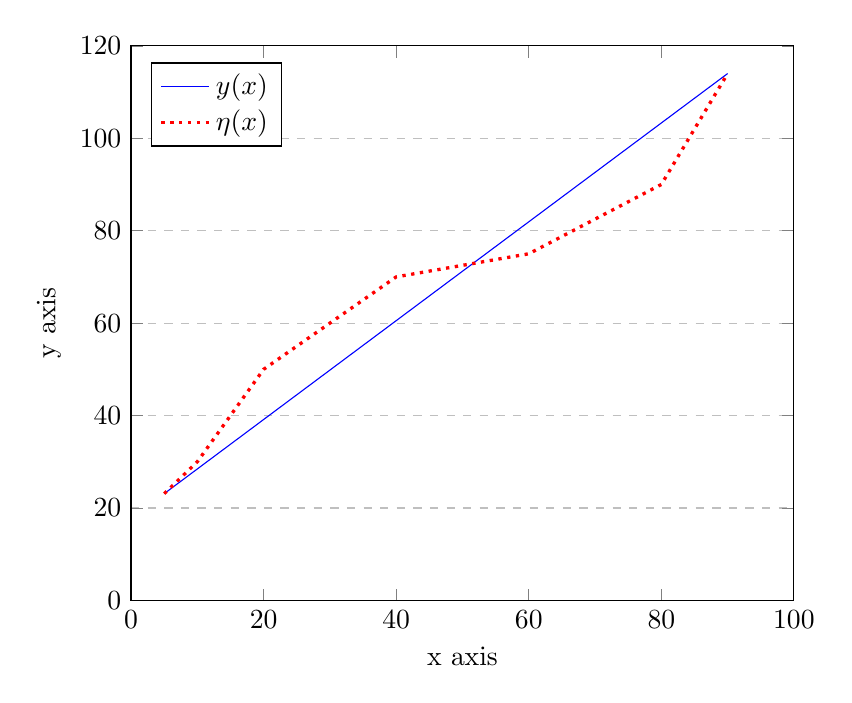
\begin{tikzpicture}
\begin{axis}[
    xlabel={x axis},
    ylabel={y axis},
    xmin=0, xmax=100,
    ymin=0, ymax=120,
    xtick={0,20,40,60,80,100},
    ytick={0,20,40,60,80,100,120},
    legend pos=north west,
    ymajorgrids=true,
    grid style=dashed,
]

\addplot[smooth]
    [color = blue]
    coordinates {
    (5,23.1)(90,114)
    };
    
\addplot[very thick, dotted][color = red]
    coordinates {
    (5,23.1)(10,30)(20,50)(30,60)(40,70)(60,75)(80,90)(90,114)
    };
    \legend{\(y(x)\), \(\eta (x)\)}

\end{axis}
\end{tikzpicture}
\\
\\
Given that we are trying to minimise the distance between the start and endpoints, a and b, we can set \(I[f] = \int\limits_a^b (ds)\), where \(ds\) is the distance between the two points.
\\
\\
As we have assumed \(y(x)\) to be a straight lime, its length must also be a straight line. Hence we can calculate \(ds\) by using pythagoras' theorem:
\\
\\

\usetikzlibrary{decorations.pathreplacing}

      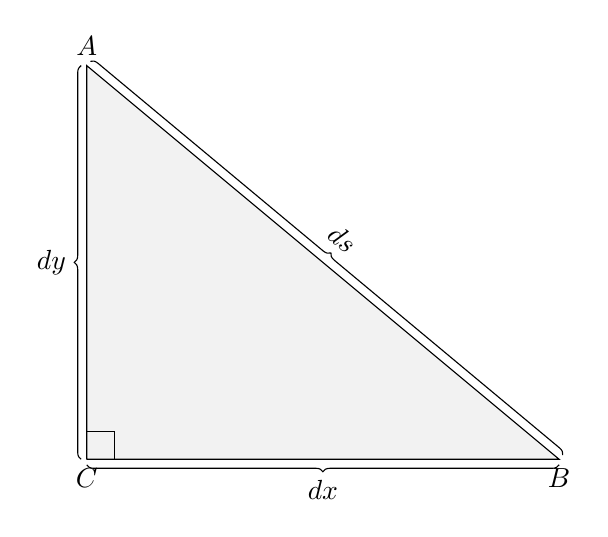
\begin{tikzpicture}
% Draw the triangle
        \draw[fill=gray!10]  (0, 0) coordinate (C) 
        -- (0,5) coordinate (A) 
        -- (6,0) coordinate (B) 
        -- (0, 0);
       \draw[decoration={brace,mirror,raise=2pt},decorate] 
         (C) -- node[below=4pt] {$dx$} (B); 
       \draw[decoration={brace,mirror,raise=2pt},decorate] 
         (B) -- node[above=4pt,sloped] {$ds$} (A); 
       \draw[decoration={brace,mirror,raise=2pt},decorate] 
         (A) -- node[left=4pt] {$dy$} (C); 

       \draw (0,10pt) -- ++(10pt,0) -- ++(0,-10pt);
% Draw nodes
        \node at (A)[anchor=south] {$A$};
        \node at (B)[anchor=north] {$B$};
        \node at (C)[anchor=north] {$C$};
      \end{tikzpicture}
\\
\\
\(ds = \sqrt{dx^2+dy^2}\)
\\
\\
\(ds = \sqrt{dx^2}\sqrt{1+(\frac{dy}{dx})^2}\)
\\
\\
\(ds = \sqrt{1+y'^2}dx\)
\\
\\
Considering our new equation for \(ds\), we can now rewrite our integral, \(I[f] = \int\limits_a^b (ds)\) as the following:
\\
\\
\(I[f] = \int\limits_a^b (\sqrt{1+y'^2}dx)\)
\\
\\
We can now recall the Euler-Lagrange equation, \(\frac{\partial F}{\partial y(x)} - \frac{d}{dx}(\frac{\partial F}{\partial y'(x)}) = 0\) to minimise \(I[f]\).
\\
\\
Given that our functional here is \(\sqrt{1+y'^2}\), which is a function of x, y, and y', as per the foundational principle of the Calculus of Variations, and given also that the functional is only a function of y', we can show that:
\\
\\
\(\frac{\partial F}{\partial y(x)} = 0\)
\\
\implies \(\frac{d}{dx}(\frac{\partial F}{\partial y'(x)}) = 0\) for the Euler-Lagrange equation to hold.
\\
\\
Therefore by integrating both sides of \(\frac{d}{dx}(\frac{\partial F}{\partial y'(x)}) = 0\), we find that \(\frac{\partial F}{\partial y'(x)} = K\), where \(K\) is some arbitrary constant.
\\
\\
As the functional, F, is equal to \(\sqrt{1+y'^2}\), then
\\
\\
\(\frac{\partial F}{\partial y'(x)} = \frac{1}{2} \cdot 2y' \cdot \frac{1}{\sqrt{1+y'^2}} = \frac{y'}{\sqrt{1+y'^2}}\)
\\
\\
By inspection, we can tell that the only way for \(\frac{\partial F}{\partial y'(x)} = \frac{y'}{\sqrt{1+y'^2}}\) to be a constant is if \(y'\) itself a constant.
\\
\\
Therefore, we can let \(y'\) equal some arbitrary constant \(C_{1}\). Therefore we can form the differential equation \(\frac{dy}{dx} = C_{1}\)
\\
\\
We can then solve this by separating variables such that
\\
\\
\(dy = C_{1} dx\)
\\
\\
By integrating both sides,
\\
\\
\(\int dy = \int(C_{1}) dx\)
\\
\implies \(y = C_{1}x + C_{2}\), which is the equation of a straight line, as required. [11]


\section{Deriving the Beltrami Identity}
As we've stated before, in the Calculus of Variations, what we're to find is \(f(x)\), such that
\\
\\
\(I[f] = \int\limits_a^b\ F(x, y, \frac{dy}{dx})\) is stationary.
\\
\\
We do this, of course, by using the Euler-Lagrange equation we derived previously. The Beltrami Identity however applies when \(F(x, y, \frac{dy}{dx})\) does not explicitly depend on \(x\), or in other words, when \(\frac{\partial F}{\partial x} = 0\) 
\\
\\
You may be wondering why this is at all useful to us. Well the reason is that the Beltrami Identity is a nice generalisation of the Euler-Lagrange equation, for when \(\frac{\partial F}{\partial x} = 0\), that we will use to present a more simplified solution of the Brachistochrone Problem through the Calculus of Variations.
\\
\\
In the end, the Beltrami Identity states:
\\
\\
\(F-y'(x)\frac{\partial F}{\partial y'(x)} = C\) where the constant \(C\) depends, of course, on the boundary conditions.
\\
\\
We can begin this derivation by considering the Euler-Lagrange equation itself to start with:
\\
\\
\(\frac{\partial F}{\partial y(x)} - \frac{d}{dx}(\frac{\partial F}{\partial y'(x)}) = 0\)
\\
\\
Then by multiplying through both sides by \(y'(x)\),
\\
\\
\(y'(x)\frac{\partial F}{\partial y(x)} - y'(x)\frac{d}{dx}(\frac{\partial F}{\partial y'(x)}) = 0\)
\\
\\
We can now consider the functional we are trying to minimise through the foundational principle of the Calculus of Variations, \(F(x, y, y')\), where F is a function of \(x, y\) and \(y'\), and \(y, y'\) are also functions of \(x\).
\\
\\
Given that for cases where the Beltrami Identity applies, \(\frac{\partial F}{\partial x} = 0\), we can consider the total derivative of \(\frac{dF}{dx}\) through the multivariable chain rule as follows:
\\
\\
\(\frac{dF}{dx} = \frac{\partial F}{\partial x} \cdot \frac{\partial x}{\partial x} + \frac{\partial F}{\partial y(x)} \cdot \frac{\partial y(x)}{\partial x} + \frac{\partial F}{\partial y'(x)} \cdot \frac{\partial y'(x)}{\partial x}\)
\\
\\
Which simplifies to
\\
\\
\(\frac{dF}{dx} = \frac{\partial F}{\partial x} + \frac{\partial F}{\partial y(x)} y'(x) + \frac{\partial F}{\partial y'(x)}y''(x)\)
\\
\\
By taking terms onto the LHS, we end up with
\\
\\
\( \frac{\partial F}{\partial y(x)} y'(x) = \frac{dF}{dx} - \frac{\partial F}{\partial x} - \frac{\partial F}{\partial y'(x)}y''(x)\)
\\
\\
By inspecting the LHS, we notice from \(y'(x)\frac{\partial F}{\partial y(x)} - y'(x)\frac{d}{dx}(\frac{\partial F}{\partial y'(x)}) = 0\), that as \( \frac{\partial F}{\partial y(x)} y'(x) = y'(x)\frac{d}{dx}(\frac{\partial F}{\partial y'(x)})\)
\\
\\
Therefore, substituting this into the LHS, we can form the equation:
\\
\\
\(y'(x)\frac{d}{dx}(\frac{\partial F}{\partial y'(x)}) = \frac{dF}{dx} - \frac{\partial F}{\partial x} - \frac{\partial F}{\partial y'(x)}y''(x)\)
\\
\\
\implies \( \frac{dF}{dx} - \frac{\partial F}{\partial x} - \frac{\partial F}{\partial y'(x)}y''(x) - y'(x)\frac{d}{dx}(\frac{\partial F}{\partial y'(x)}) = 0\)
\\
\\
\implies \( \frac{dF}{dx} - \frac{\partial F}{\partial x} - (\frac{\partial F}{\partial y'(x)}y''(x) + y'(x)\frac{d}{dx}(\frac{\partial F}{\partial y'(x)})) = 0\)
\\
\\
By noticing that the expression inside of the brackets can be simplified through reverse product rule, where
\\
\\
\(\frac{\partial F}{\partial y'(x)}y''(x) + y'(x)\frac{d}{dx}(\frac{\partial F}{\partial y'(x)}) = \frac{d}{dx}y'(x)\frac{\partial F}{\partial y'(x)}\)
\\
\\
Therefore, we can rewrite the equation as
\\
\\
\( \frac{dF}{dx} - \frac{\partial F}{\partial x} - \frac{d}{dx}y'(x)\frac{\partial F}{\partial y'(x)} = 0\)
\\
\\
Now given that the Beltrami Identity only applies to functionals which do not explicitly depend on \(x\), or rather where \(\frac{\partial F}{\partial x} = 0\), we can rearrange the equation to place \(\frac{\partial F}{\partial x}\) by itself on one side, and the rest of the terms on another as follows:
\\
\\
\( \frac{\partial F}{\partial x} = \frac{dF}{dx} - \frac{d}{dx}y'(x)\frac{\partial F}{\partial y'(x)}\)
\\
\\
\implies \( \frac{\partial F}{\partial x} = \frac{d}{dx}(F - y'(x)\frac{\partial F}{\partial y'(x)})\)
\\
\\
Now as \( \frac{\partial F}{\partial x} = 0\), we can rewrite this as
\\
\\
\(\frac{d}{dx}(F - y'(x)\frac{\partial F}{\partial y'(x)}) = 0\)
\\
\\
By integrating both sides with respect to \(x\), we arrive at the Beltrami Identity:
\\
\\
\(F - y'(x)\frac{\partial F}{\partial y'(x)} = C\),
\\
\\
for some arbitrary constant \(C\) that depends on boundary conditions. [12]
\section{Proof Through The Calculus of Variations}
We've reached our point of culmination. Proving the correct solution to the Brachistochrone Problem using the Calculus of Variations. I will restate the Brachistochrone Problem for convenience's sake:
\\
\\
"Given 2 points, A and B, in an \(x-y\) plane, what is the curve traced out by a point acted on only by gravity, which starts at A and reaches B in the shortest time?" [1]
\\
\\
The solution below will utilise everything introduced in the previous chapter, including the Euler-Lagrange equation and the Beltrami Identity. It will also make use of conservation of energy to lead us to a differential equation unveiling the parametric equations of the cycloid as our final answer.
\\
\\
To begin our proof, we can consider the following diagram:
\\
\\
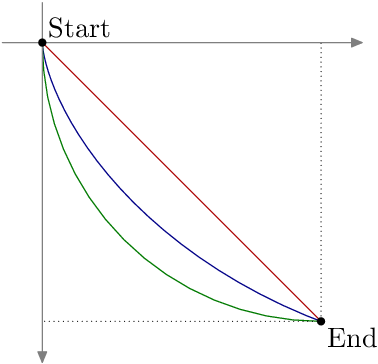
\includegraphics[width=9cm, height=7cm]{EPQ - VC/3.5 Diag.png}
\\
\\
Here we can let the start and endpoints be a and b respectively. We can also assume that the particle starts at a, and is acted on only by gravity, and is not affected by air resistance or any other frictional or resistive forces.
\\
\\
What we are trying to do is set some integral \(I[f]\) that minimises the time taken for the particle to travel from a to b. This is what will help us find the equation of the curve traced out by the particle travelling subject to these constraints.
\\
\\
We can first consider \(I[f] = \int\limits_0^t (dt)\) as this calculates the total time taken to travel from rest, from a to b. This is what we are looking to minimise. However, for the sake of producing an integrable functional which will reveal the equation of the curve formed by the path of the particle, we can rewrite the time taken, \(dt\), in terms of the path length, \(ds\) and the velocity, \(v\).
\\
\\
As \(speed = \frac{distance}{time}\), \(v = \frac{ds}{dt}\), and hence \(dt = \frac{ds}{v}\).
\\
\\
We can now rewrite \(I[f]\), however we must consider the limits before doing so. Given that at time = 0, the particle is still at the start point, and hence still at a, and at time = t, the particle is at the endpoint, and hence at b, we can rewrite the limits, 0 and t, of \(I[f]\) as a and b respectively, as we make the substitution \(dt = \frac{ds}{v}\).
\\
\\
Therefore we can now rewrite \(I[f] = \int\limits_0^t (dt)\) as \(I[f] = \int\limits_a^b \frac{ds}{v}\)
\\
\\
By noting that the only force acting on the particle is gravity, we can use conservation of energy to rewrite \(v\) as follows:
\\
\\
\(\frac{1}{2}mv^2 = mg\Delta h\)
\\
\\
\implies \(v = \sqrt{2g\Delta h}\)
\\
\\
Therefore, by substituting for \(v\), \((I[f] = \int\limits_a^b \frac{ds}{\sqrt{2g\Delta h}}\)
\\
\\
We can also recall from (3.3) that \(ds = \sqrt{1+y'^2} dx\), therefore we further substitute this value into \(I[f]\), to form an integral that can be solved via the Euler-Lagrange equation. This is because the resulting integral will be only in terms of \(x, y\) and \(y'\), and hence the Euler-Lagrange equation can be applied to the functional we are looking to minimise. 
\\
\\
Substituting for \(ds\), \(I[f] = \int\limits_a^b \frac{\sqrt{1+y'^2} dx}{\sqrt{2g\Delta h}}\)
\\
\\
\implies \(I[f] = \frac{1}{\sqrt{2g}}\int\limits_a^b \frac{\sqrt{1+y'^2} dx}{\sqrt{y}}\) ,
\\
\\
as \(\Delta h\) = the height the particle falls = \(y\).
\\
\\
Now given that by inspection we can identify that the functional, \(F = \frac{\sqrt{1+y'^2} dx}{\sqrt{y}}\) does not explicitly depend on \(x\), we can apply the Beltrami Identity, a special case of the Euler-Lagrange equation where the functional does not explicitly depend on \(x\).
\\
\\
We can recall the Beltrami Identity to be \(F - y'(x)\frac{\partial F}{\partial y'(x)} = C\)
\\
\\
By substituting in our value of \(F\) into the Beltrami Identity, we find:
\\
\\
\(\sqrt{\frac{{1+y'^2}}{y}} - y' \cdot \frac{1}{\sqrt{y}} \cdot \frac{1}{2\sqrt{1+y'^2}} \cdot 2y' = C\)
\\
\\
\implies \(\sqrt{\frac{{1+y'^2}}{y}} - \frac{y'^2}{\sqrt{y(1+y'^2)}} = C\)
\\
\\
Multiplying through both sides by \(\sqrt{y}\) \implies \(\sqrt{1+y'^2} - \frac{y'^2}{\sqrt{1+y'^2}} = C\sqrt{y}\)
\\
\\
Now multiplying through both sides by \(\sqrt{1+y'^2}\)
\\
\(\implies 1 + y'^2 - y'^2 = C\sqrt{y(1+y'^2)}\)
\\
\\
\implies \(C\sqrt{y(1+y'^2)} = 1\)
\\
\\
By squaring both sides \implies \(C^2(y(1+y'^2)) = 1\)
\\
\\
\implies \(y(1+y'^2) = \frac{1}{C^2}\)
\\
\\
As \(\frac{1}{C^2}\) is a constant, we can let it equal some arbitrary constant \(C_{1}\)
\\
\implies \(y(1+y'^2) = C_{1}\)
\\
\\
\(y+y \cdot y'^2 = C_{1}\)
\\
\\
By rearranging this equation to make \(y'\) the subject,
\\
\\
\(y'^2 = \frac{C_{1}-y}{y}\)
\\
\\
Therefore \(y' = \sqrt{\frac{C_{1}-y}{y}}\)
\\
\\
And hence, \(\frac{dy}{dx} = \sqrt{\frac{C_{1}-y}{y}}\)
\\
\\
We can notice here that this is the differential equation we solved in chapter (2.3).
\\
\\
By solving this using exactly the same methods shown in (2.3), we arrive at the solutions:
\\
\\
\(x = C_{1} (\theta-\frac{1}{2}\sin{2\theta}) - C_{2}\)
\\
\\
\(y =\frac{C_{1}}{2} \cdot (1-\cos{2\theta}) \)
\\
\\
Where \(C_{1}\) and \(C_{2}\) are of course arbitrary constants which can be determined by the boundary conditions.
\\
\\
These set of parametric equations, as shown in the previous chapter, are known to resemble those of the Cycloid. Hence we can conclude that the final shape of the path taken by the particle, where the path is such that the time taken from a to b is minimised, is the shaped traced out by a point on a Cycloid moving moving between the 2 points.
\\
\\
We can again further consult the diagram below for a more geometrical perspective of the solution:
\\
\\
\begin{tikzpicture}
\draw[->] (0,0) -- (0,3);
\draw[->] (0,0) -- (2.6*pi,0);
\draw[red,domain=-0.5*pi:2.5*pi,samples=50] plot ({\x - sin(\x r)},{1 - cos(\x r)});
\end{tikzpicture} [4]
\chapter{Bibliography}
\begin{itemize}
    \item [1]  St. Andrew's University, School of Mathematics and Statistics (2002). The Brachistochrone Problem.
    Authors: J J O'Connor and E F Robertson
    \\
    URL: https://mathshistory.st-andrews.ac.uk/HistTopics/Brachistochrone/
    \\
    Date Accessed: 05/09/2021
    \item [2] Tex StackExchange (2020). Illustrating Newton's Path of Fastest Descent. 
    Author: Thruston (username on website)
    \\
    URL: https://tex.stackexchange.com/questions/568105/illustrating-newtons-path-of-fastest-descent
    \\
    Date Accessed: 2/12/2021
    \item [3] Mathematical Association of America (2014). Historical Activities for Calculus - Module 3: Optimization – Galileo and the Brachistochrone Problem.
    Author: Gabriela R. Sanchis (Elizabethtown College)
    \\
    URL: https://www.maa.org/press/periodicals/convergence/historical-activities-for-calculus-module-3-optimization-galileo-and-the-brachistochrone-problem
    \\
    Date Accessed: 05/09/2021
    \item [4] YouTube (2021). The Brachistochrone Problem. Author: Good Vibrations with Freeball (YouTube Channel)
    \\
    URL: https://www.youtube.com/watch?v=3HXCv4dmR7A
    \\
    Date Accessed: 10/11/2021
    \item [5] UC Santa Cruz Department of Physics (2009). Fermat’s Principle and the Laws of Reflection and Refraction. Author: Professor Howard Haber
    \\
    URL: http://scipp.ucsc.edu/~haber/ph5B/fermat09.pdf (1)
    \\
    Date Acessed: 07/09/2021
    \item [6] Johann Bernoulli Institute, University of Groningen (2014). Bernoulli’s light ray solution of the brachistochrone problem through Hamilton’s eyes. Author: Henk W. Broer
    \\
    URL: https://www.math.rug.nl/~broer/pdf/ws-ijbc.pdf (3-4)
    \\
    Date Acessed: 17/10/2021
    \item [7] Massachusetts Institute of Technology (2010). General Parametric Equations; the Cycloid. Author: Prof. Denis Auroux
    \\
    URL: https://ocw.mit.edu/courses/18-02sc-multivariable-calculus-fall-2010/ (Vectors and Matrices/ Part C/ Session 17: General Parametric Equations; the Cycloid /Reading and Examples, 3)
    \\
    Date Accessed: 20/09/2021
    \item [8] Department of Engineering Science and Physics, The College of Staten Island, The City University of New York, Staten Island (1999). Author: Herman Erlichson
    \\
    URL: https://mecheng.iisc.ac.in/suresh/me256/GalileoBP.pdf
    \\
    Date Acessed: 18/10/2021
    \item [9] Department of Physics, Virginia Tech (2019). The Tautochrone/Brachistochrone Problems: How to make the Period of a Pendulum independent of its Amplitude. Author: Tatsu Takeuchi
    \\
    URL: http://www1.phys.vt.edu/~takeuchi/Tools/CSAAPT-Fall2019-takeuchi.pdf (5)
    \\
    Date Accessed: 10/11/2021
    \item [10] YouTube (2020). Introduction to Variational Calculus - Deriving the Euler-Lagrange Equation. Author: Good Vibrations with Freeball (YouTube Channel)
    \\
    URL: https://www.youtube.com/watch?v=VCHFCXgYdvY&t=348s
    \\
    Date Accessed: 10/11/2021
    \item [11] YouTube (2021). Shortest Distance Path Between Two Points On A Plane. Author: Good Vibrations with Freeball (YouTube Channel)
    \\
    URL: https://www.youtube.com/watch?v=YVLFHE-mJ7w
    \\
    Date Acessed: 19/11/2021
    \item [12] YouTube (2017). Beltrami Identity Derivation | Calculus of Variations. Author: Faculty of Khan (YouTube Channel)
    \\
    URL: https://www.youtube.com/watch?v=tm17eLIObdA
    \\
    Date Accessed: 2/12/2021
    \item [13] Technion - Israel institute of technology (2020). Research and analysis of the various solutions provided for the Brachistochrone problem. Author: Ido Braun
    \\
    https://aerospace.technion.ac.il/wp-content/uploads/2020/07/Full-Report-14.7.pdf
    \\
    Date Accessed: 8/12/2021
    \item [14] University of Montana (2008). "The Brachistochrone Problem: Mathematics for a Broad Audience via a Large Context Problem," The Mathematics Enthusiast: Vol. 5 : No. 2 , Article 2. Authors: Jeff Babb and James Currie
    \\
    URL: https://scholarworks.umt.edu/cgi/viewcontent.cgi?article=1099&context=tme#:~:text=In
    \\
    Date Accessed: 17/10/2021
    \item [15] Tex StackExchange (2014). How can I draw this cycloid diagram with TikZ?. Author: Herman Jaramillo
    \\
    URL: https://tex.stackexchange.com/questions/196957/how-can-i-draw-this-cycloid-diagram-with-tikz
    \\
    Date Accessed: 15/09/2021
\end{itemize}

\end{document}


